\documentclass[wide,a4paper,titlepage,12pt] {article}
\usepackage{polski}
\usepackage[UTF8]{inputenc}
\usepackage{listings}
\usepackage{slashbox}
\usepackage[table]{xcolor}
\usepackage{graphicx,pdflscape}
\usepackage{placeins}


\title{Grafika komputerowa}
\author{Jacek Wieczorek (181043)}

% Title page layout (fold)
\makeatletter
\renewcommand{\maketitle}{
\begin{titlepage}
  \begin{center}
    \vspace*{3cm}
    \LARGE \@title \par
    \vspace{2cm}
    \textit{\small Autor:}\par
    \normalsize \@author\par \normalsize
    \vspace{3cm}
    \textit{\small Prowadzący:}\par
    Dr inż. Tomasz Kapłon \par
    \vspace{2cm}
    Wydział Elektroniki\\ III rok\\ Pn TP 08.15 - 11.00\par
    \vspace{4cm}
    \small \@date
  \end{center}
\end{titlepage}
}
\makeatother
% Title page layout (end)



\begin{document}
\maketitle
  \section{Cel laboratorium}
	Celem ćwiczenia jest wprowadzenie w zagadnienia modelowania i wizualizacji scen $3D$ z wykorzystaniem biblioteki OpenGL z rozszerzeniem GLUT. Modelowanym przez nas obiektem jest jajko, opisane następującymi równaniami parametrycznymi : \\
\begin{figure}[htbp]
	 		\begin{center}
         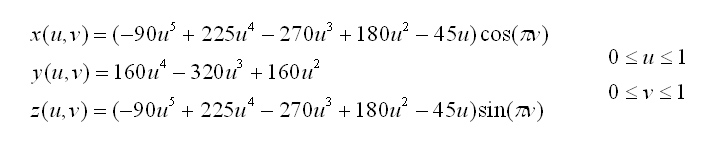
\includegraphics[scale=0.6]{row.jpg}
      %\caption{}
     \end{center}
     \end{figure}
  \\ Pętla odpowiedzialna za wyliczenie punktów jajka w przestrzeni $3D$ :\\
\lstset{ %
    language=c++,                % choose the language of the code
    basicstyle=\scriptsize,       % the size of the fonts that are used for the code
    numbers=left,                   % where to put the line-numbers
    numberstyle=\scriptsize,      % the size of the fonts that are used for the line-numbers
    stepnumber=10,                   % the step between two line-numbers. If it's 1 each line 
                                    % will be numbered
    numbersep=9pt,                  % how far the line-numbers are from the code
    % backgroundcolor=\color{white},  % choose the background color. You must add \usepackage{color}
    showspaces=false,               % show spaces adding particular underscores
    showstringspaces=false,         % underline spaces within strings
    showtabs=false,                 % show tabs within strings adding particular underscores
    % frame=single,                 % adds a frame around the code
    % tabsize=2,                  % sets default tabsize to 2 spaces
    % captionpos=b,                   % sets the caption-position to bottom
    breaklines=true,                % sets automatic line breaking
    % breakatwhitespace=false,        % sets if automatic breaks should only happen at whitespace
    % title=\lstname,                 % show the filename of files included with \lstinputlisting;
                                    % also try caption instead of title
    % escapeinside={\%*}{*)},         % if you want to add a comment within your code
    % morekeywords={*,...}            % if you want to add more keywords to the set
    }
    \lstinputlisting{row.cpp}
\newpage
\section{Wyświetlanie jajka jako zbiór punktów}
Pierwszym zadaniem było wyświetlenie jajka jako zbioru punktów w przestrzeni $3D$.\\
Funkcja odpowiedzialna za wyświetlanie jajka : \\
\lstset{ %
    language=c++,                % choose the language of the code
    basicstyle=\scriptsize,       % the size of the fonts that are used for the code
    numbers=left,                   % where to put the line-numbers
    numberstyle=\scriptsize,      % the size of the fonts that are used for the line-numbers
    stepnumber=10,                   % the step between two line-numbers. If it's 1 each line 
                                    % will be numbered
    numbersep=9pt,                  % how far the line-numbers are from the code
    % backgroundcolor=\color{white},  % choose the background color. You must add \usepackage{color}
    showspaces=false,               % show spaces adding particular underscores
    showstringspaces=false,         % underline spaces within strings
    showtabs=false,                 % show tabs within strings adding particular underscores
    % frame=single,                 % adds a frame around the code
    % tabsize=2,                  % sets default tabsize to 2 spaces
    % captionpos=b,                   % sets the caption-position to bottom
    breaklines=true,                % sets automatic line breaking
    % breakatwhitespace=false,        % sets if automatic breaks should only happen at whitespace
    % title=\lstname,                 % show the filename of files included with \lstinputlisting;
                                    % also try caption instead of title
    % escapeinside={\%*}{*)},         % if you want to add a comment within your code
    % morekeywords={*,...}            % if you want to add more keywords to the set
    }
    \lstinputlisting{j1.cpp}

\begin{figure}[htbp]
	 		\begin{center}
         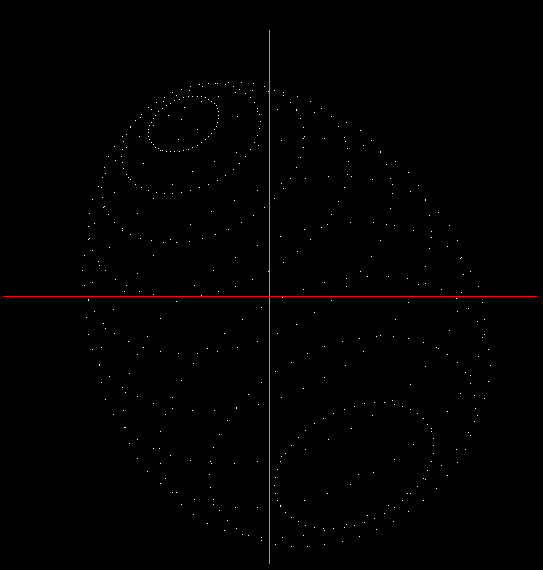
\includegraphics[scale=0.7]{j1.PNG}
      \caption{Jajko dla N=25 }
     \end{center}
     \end{figure}
\newpage
\section{Jajko jako siatka}
Kolejnym zadaniem było połączenie punktów jajka i narysowanie go jako siatki południków i równoleżników. Zadanie wymagało połączenia ze soba odpowiednich punktów za pomocą konstrukcjii $glBegin(GL\_LINES); ... glEnd()$.\\
Funkcja odpowiedzialna za rysowanie siatki : \\
\lstset{ %
    language=c++,                % choose the language of the code
    basicstyle=\scriptsize,       % the size of the fonts that are used for the code
    numbers=left,                   % where to put the line-numbers
    numberstyle=\scriptsize,      % the size of the fonts that are used for the line-numbers
    stepnumber=10,                   % the step between two line-numbers. If it's 1 each line 
                                    % will be numbered
    numbersep=9pt,                  % how far the line-numbers are from the code
    % backgroundcolor=\color{white},  % choose the background color. You must add \usepackage{color}
    showspaces=false,               % show spaces adding particular underscores
    showstringspaces=false,         % underline spaces within strings
    showtabs=false,                 % show tabs within strings adding particular underscores
    % frame=single,                 % adds a frame around the code
    % tabsize=2,                  % sets default tabsize to 2 spaces
    % captionpos=b,                   % sets the caption-position to bottom
    breaklines=true,                % sets automatic line breaking
    % breakatwhitespace=false,        % sets if automatic breaks should only happen at whitespace
    % title=\lstname,                 % show the filename of files included with \lstinputlisting;
                                    % also try caption instead of title
    % escapeinside={\%*}{*)},         % if you want to add a comment within your code
    % morekeywords={*,...}            % if you want to add more keywords to the set
    }
    \lstinputlisting{j2.cpp}

\begin{figure}[htbp]
	 		\begin{center}
         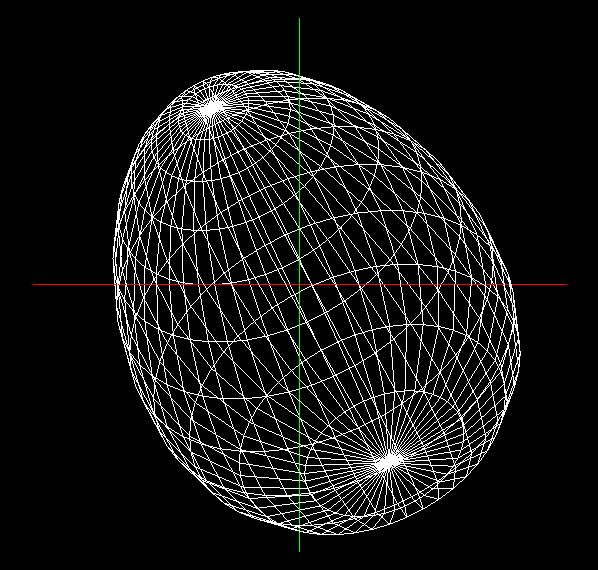
\includegraphics[scale=0.65]{j2.PNG}
      \caption{Jajko dla N=25 }
     \end{center}
     \end{figure}
\newpage
\section{Jajko jako zbiór trójkątów}
Ostatnim zadaniem było narysowanie jajka jako zbiór trójkątów o losowo wybranych kolorach. Metoda ta powodowała, że narysowane jajko ma tzw. "szew" biegnący wzdłóż jego połówek. W celu wyeliminowania problemu, należało wartością kolorów skrajnych trójkątów połówek jajka nadać ten sam kolor. Dotakowym problemem okazał się fakt, że dla sąsiadujące ze sobą połówek, skrajne indeksy $i$ mają inne wartości, a mianowicie $i \rightarrow( N-i-1)$. Dzięki temu otrzymywaliśmy efekt płynnego przejścia kolorów i jednolitą powierzchnię.\\ \\
Funkcja losująca kolory i eliminująca szew : 
\lstset{ %
    language=c++,                % choose the language of the code
    basicstyle=\scriptsize,       % the size of the fonts that are used for the code
    numbers=left,                   % where to put the line-numbers
    numberstyle=\scriptsize,      % the size of the fonts that are used for the line-numbers
    stepnumber=10,                   % the step between two line-numbers. If it's 1 each line 
                                    % will be numbered
    numbersep=9pt,                  % how far the line-numbers are from the code
    % backgroundcolor=\color{white},  % choose the background color. You must add \usepackage{color}
    showspaces=false,               % show spaces adding particular underscores
    showstringspaces=false,         % underline spaces within strings
    showtabs=false,                 % show tabs within strings adding particular underscores
    % frame=single,                 % adds a frame around the code
    % tabsize=2,                  % sets default tabsize to 2 spaces
    % captionpos=b,                   % sets the caption-position to bottom
    breaklines=true,                % sets automatic line breaking
    % breakatwhitespace=false,        % sets if automatic breaks should only happen at whitespace
    % title=\lstname,                 % show the filename of files included with \lstinputlisting;
                                    % also try caption instead of title
    % escapeinside={\%*}{*)},         % if you want to add a comment within your code
    % morekeywords={*,...}            % if you want to add more keywords to the set
    }
    \lstinputlisting{szew.cpp}
 Funkcja rysująca jajko : 
\lstset{ %
    language=c++,                % choose the language of the code
    basicstyle=\scriptsize,       % the size of the fonts that are used for the code
    numbers=left,                   % where to put the line-numbers
    numberstyle=\scriptsize,      % the size of the fonts that are used for the line-numbers
    stepnumber=10,                   % the step between two line-numbers. If it's 1 each line 
                                    % will be numbered
    numbersep=9pt,                  % how far the line-numbers are from the code
    % backgroundcolor=\color{white},  % choose the background color. You must add \usepackage{color}
    showspaces=false,               % show spaces adding particular underscores
    showstringspaces=false,         % underline spaces within strings
    showtabs=false,                 % show tabs within strings adding particular underscores
    % frame=single,                 % adds a frame around the code
    % tabsize=2,                  % sets default tabsize to 2 spaces
    % captionpos=b,                   % sets the caption-position to bottom
    breaklines=true,                % sets automatic line breaking
    % breakatwhitespace=false,        % sets if automatic breaks should only happen at whitespace
    % title=\lstname,                 % show the filename of files included with \lstinputlisting;
                                    % also try caption instead of title
    % escapeinside={\%*}{*)},         % if you want to add a comment within your code
    % morekeywords={*,...}            % if you want to add more keywords to the set
    }
    \lstinputlisting{j3.cpp}
\newpage
\begin{figure}[htbp]
	 		\begin{center}
         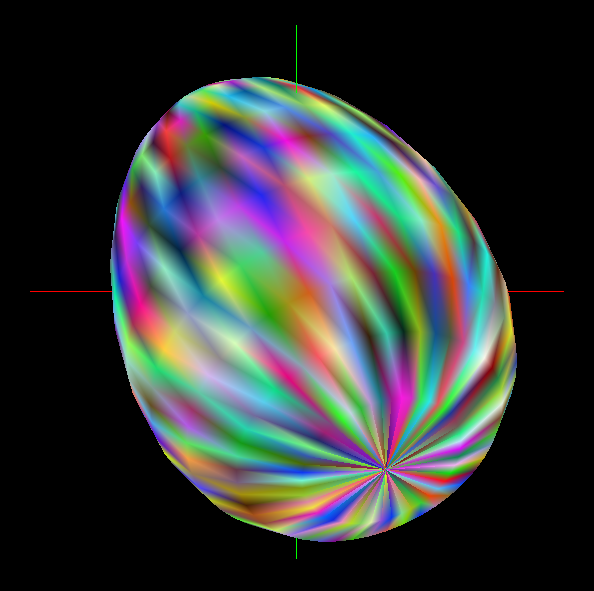
\includegraphics[scale=0.65]{j3.PNG}
      \caption{Jajko dla N=25 }
     \end{center}
     \end{figure}
\section{Dodatkowe funkcjonalności}
Dodatkowe funkcjonalności zaimplementowane w programie :
\begin{itemize}
	\item Wybór trybu jajka : trójkąty, siatka, punkty jako odpowiednio lawisze klawiatury : $s$, $w$, $p$
	\item Ruch jajka 
\end{itemize}
Funkcje odpowiadjące za powyższe funkcjonalności :
\lstset{ %
    language=c++,                % choose the language of the code
    basicstyle=\scriptsize,       % the size of the fonts that are used for the code
    numbers=left,                   % where to put the line-numbers
    numberstyle=\scriptsize,      % the size of the fonts that are used for the line-numbers
    stepnumber=10,                   % the step between two line-numbers. If it's 1 each line 
                                    % will be numbered
    numbersep=9pt,                  % how far the line-numbers are from the code
    % backgroundcolor=\color{white},  % choose the background color. You must add \usepackage{color}
    showspaces=false,               % show spaces adding particular underscores
    showstringspaces=false,         % underline spaces within strings
    showtabs=false,                 % show tabs within strings adding particular underscores
    % frame=single,                 % adds a frame around the code
    % tabsize=2,                  % sets default tabsize to 2 spaces
    % captionpos=b,                   % sets the caption-position to bottom
    breaklines=true,                % sets automatic line breaking
    % breakatwhitespace=false,        % sets if automatic breaks should only happen at whitespace
    % title=\lstname,                 % show the filename of files included with \lstinputlisting;
                                    % also try caption instead of title
    % escapeinside={\%*}{*)},         % if you want to add a comment within your code
    % morekeywords={*,...}            % if you want to add more keywords to the set
    }
    \lstinputlisting{rest.cpp}
\section{Wnioski}
Laboratorium pozwoliło zapoznać się z podstawami modelowania obiektów w przetrzeni $3D$. Nie jest to łatwe zadanie wymagające dużej wiedzy z zakresu matematyki i grafiki komputerowej.
\end{document}